\documentclass[final,hyperref={pdfpagelabels=false}]{beamer}
\usetheme{umbc4}
\useinnertheme{umbcboxes}
\setbeamercolor{umbcboxes}{bg=violet!15,fg=black}
\usepackage{grffile}
\mode<presentation>{\usetheme{I6pd2}}
\usepackage[english]{babel}
\usepackage[latin1]{inputenc}
\usepackage{amsmath,amsthm, amssymb, latexsym}
\usepackage{subfig}
%\usepackage{times}\usefonttheme{professionalfonts}  % obsolete
%\usefonttheme[onlymath]{serif}
\boldmath
\usepackage[orientation=portrait,size=ua,scale=1.4,debug]{beamerposter}
\usepackage{ragged2e} 
\usepackage{bm}
% change list indention level
% \setdefaultleftmargin{3em}{}{}{}{}{}

%\usepackage{snapshot} % will write a .dep file with all dependencies, allows for easy bundling


\usepackage{array,booktabs,tabularx}
\newcolumntype{R}{>{\centering\arraybackslash}X} % right justified tabularx columns
\newcommand{\pphantom}{\textcolor{ta3aluminium}} % phantom introduces a vertical space in p formatted table columns??!!
\newcommand{\p}{\partial}
\newcommand{\bu}{\bm{u}}
\newcommand{\bv}{\bm{v}}
\newcommand{\imag}{\operatorname{Im}}

\listfiles

%%%%%%%%%%%%%%%%%%%%%%%%%%%%%%%%%%%%%%%%%%%%%%%%%%%%%%%%%%%%%%%%%%%%%%%%%%%%%%%%%%%%%%
\graphicspath{{figures/}}
 
\title{{\huge Non-ideal gravitational instabilities in protoplanetary disks}} 
\author{Min-Kai Lin and Kaitlin M. Kratter}
% \institute[UA]{Steward Observatory, 933 N Cherry Avenue,
%   Tucson, AZ, 85721, USA}
\institute[UA]{minkailin@email.arizona.edu, kkratter@email.arizona.edu}
%% \date[Sep. 8th, 2009]{Sep. 8th, 2009}

%%%%%%%%%%%%%%%%%%%%%%%%%%%%%%%%%%%%%%%%%%%%%%%%%%%%%%%%%%%%%%%%%%%%%%%%%%%%%%%%%%%%%%
\newlength{\columnheight}
\setlength{\columnheight}{105cm}
\setbeamertemplate{caption}{\centering\insertcaption\par}

%%%%%%%%%%%%%%%%%%%%%%%%%%%%%%%%%%%%%%%%%%%%%%%%%%%%%%%%%%%%%%%%%%%%%%%%%%%%%%%%%%%%%%
\begin{document}

\captionsetup[subfigure]{labelformat=empty}

\begin{frame}
  \begin{columns}
    % ---------------------------------------------------------%
    % Set up a column 
    \begin{column}{.49\textwidth}
      \begin{beamercolorbox}[center,wd=\textwidth]{postercolumn}
        \begin{minipage}[T]{.95\textwidth}  % tweaks the width, makes a new \textwidth
          \parbox[t][\columnheight]{\textwidth}{ % must be some better way to set the the height, width and textwidth simultaneously
            % Since all columns are the same length, it is all nice and tidy.  You have to get the height empirically
            % ---------------------------------------------------------%
            % fill each column with content            
            \begin{block}{{\Large Introduction}}
              \justifying
              {\large              
                {\bf
                  The self-gravitational fragmentaion of massive
                  proto-planetary/stellar disks is a potential
                  route to the formation of giant planets, brown
                  dwarfs or sub-stellar companions on wide
                  orbits. This phenomenon is usually studied via
                  direct numerical simluations, which may include a
                  range of physical 
                  effects such as cooling, turbulence and 
                  irradiation. However, these simulations are also
                  subject to uncertainties associated with their 
                  numerical setups. We circumvent this difficulty by
                  extending the   
                  analytic treatment of gravitational instabilities 
                  to include the above non-ideal physics, thereby 
                  predict disk fragmentation \emph{without}
                  input from previous numerical simulations. 
                }
              }
            \end{block}
            
            
            \begin{block}{{\Large Fragmentation criteria for PPDs}}
              \justifying
              \begin{center}
                \begin{onlinebox}{6.5cm}
                  \[ Q\equiv\frac{c_s\Omega}{\pi G \Sigma}\lesssim 2\] 
                \end{onlinebox}
                and
                \begin{onlinebox}{4.5cm}
                  \[t_\mathrm{cool}\Omega\lesssim 3\]
                \end{onlinebox}
              \end{center}
              The \textcolor{blue}{\it cooling criterion} ($\leftrightarrow$ a viscosity criterion) is   
              \begin{itemize}
              \item {\bf Empirical} --- observed in numerical
                simulations,  no analytical basis
              \item Possibly dependent on numerical setup of the simulation!
              \end{itemize}
              \begin{figure}
                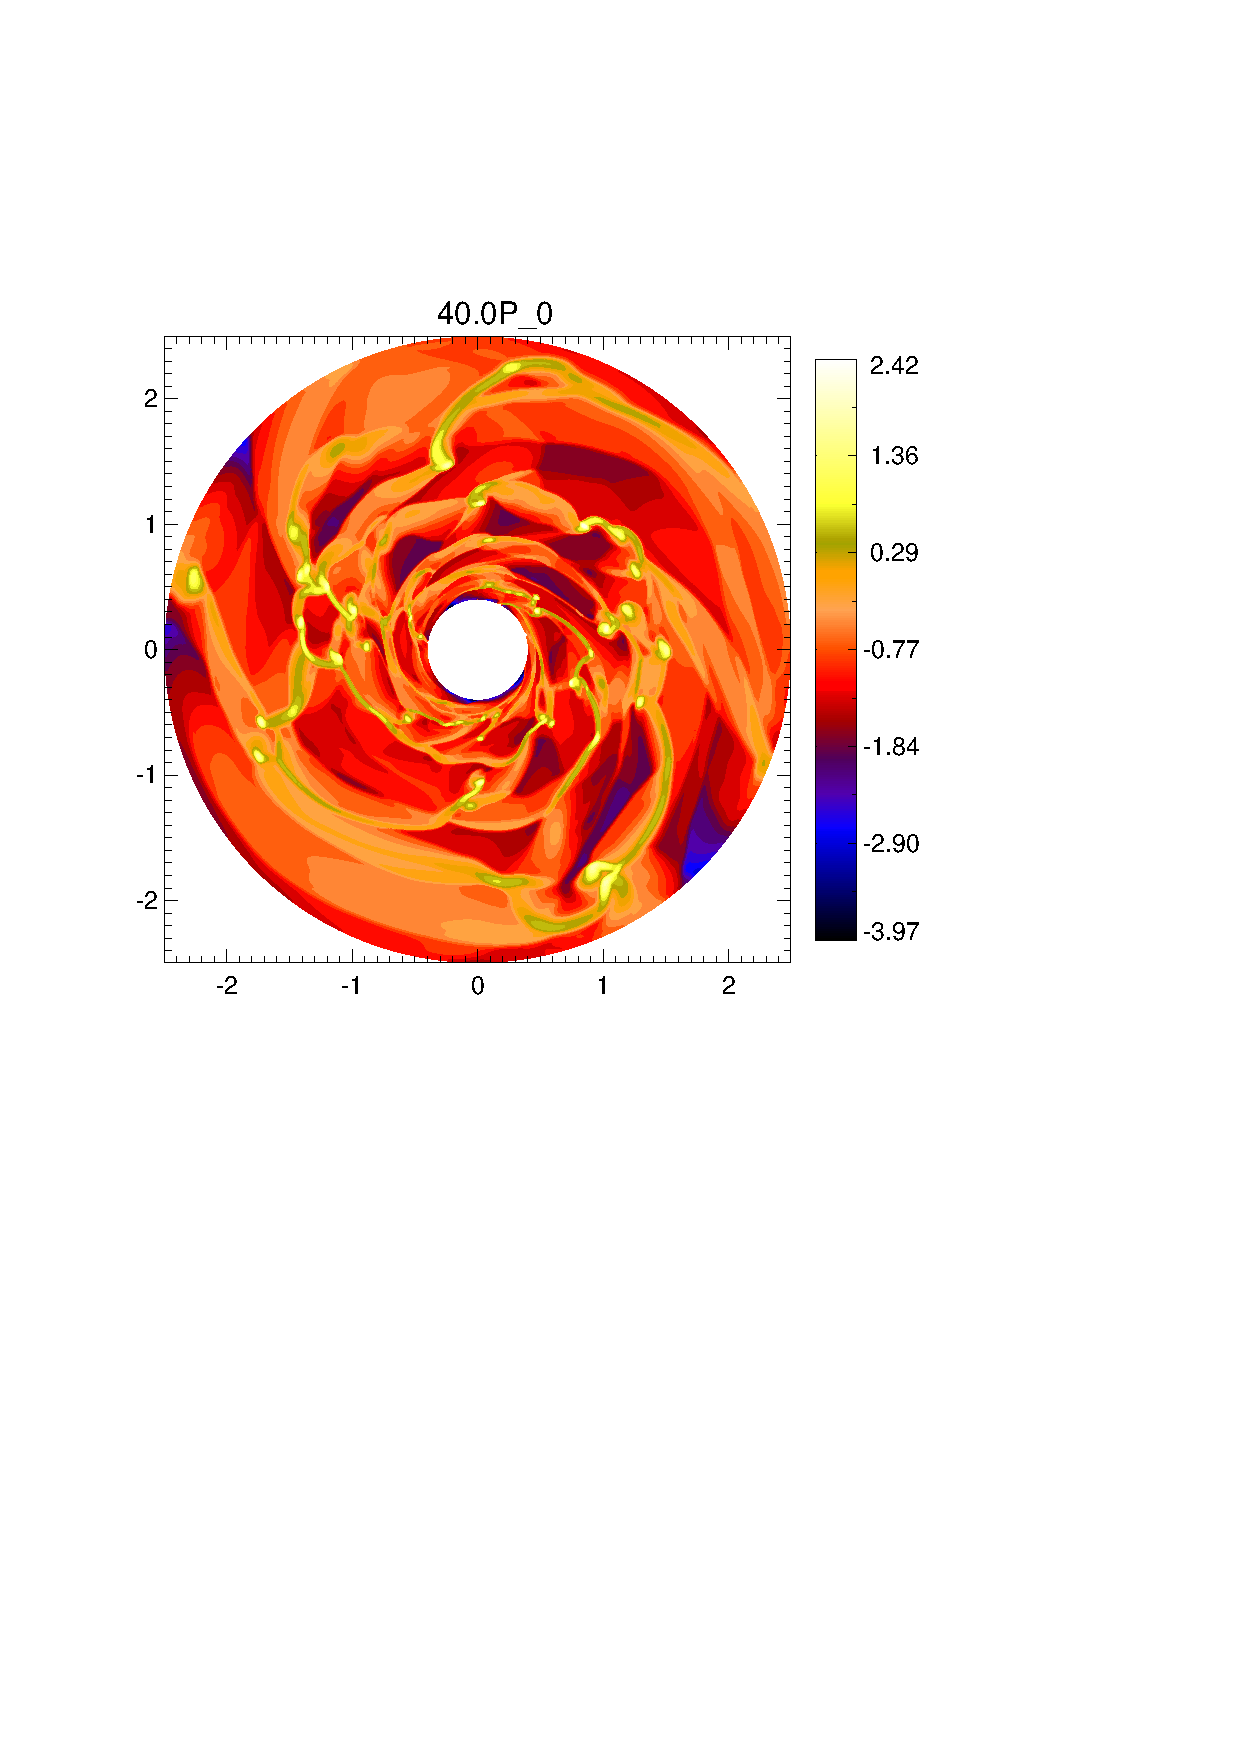
\includegraphics[width=\linewidth,clip=true,trim=0cm 0cm 0cm 0.6cm]{figures/disk_frag1}
              \end{figure}
            (Fargo simulation, $\log \Sigma$ shown)
            \end{block}
            
            \begin{block}{{\Large Simulations v.s. classic analyses}}
              \justifying
             % \centering {\large \bf{Significant mismatch!}}\\
              \begin{minipage}[t]{0.49\linewidth}
                \centering \begin{onlinebox}{5cm}Modern sims.\end{onlinebox}
                  (c. 2010)
                  \begin{itemize}
                  \item Have \textcolor{blue}{cooling physics}, 
                    \[
                    \frac{\p E}{\p t} = - \frac{E}{\color{blue}{t_\mathrm{cool}}}
                    \]
                    %\item Irradiation
                  \item Are turbulent/\textcolor{red}{viscous}, 
                    \[
                    \nu = {\color{red}{\alpha}}\frac{c_s^2}{\Omega}
                    \]
                  \end{itemize}
              \end{minipage}
              \begin{minipage}[t]{0.49\linewidth}
                \centering \begin{onlinebox}{6cm}Analytic toolbox\end{onlinebox}
                  (c. 1960) \\
                  \begin{itemize}
                  \item No cooling 
                    \[
                    \frac{\p E}{\p t} = 0
                    \]
                  \item Laminar 
                    \[
                    \nu = 0
                    \]
                  \item $\omega^2= \Omega^2 - 2\pi G \Sigma |k| +
                    c_s^2k^2 $
                  \end{itemize}
              \end{minipage}\\
              \vspace{1cm}
            
              \centering {\bf Classic  $\omega^2(k,Q)$ cannot capture cooling/viscous effects!}
              
            \end{block}
            
            
            \begin{block}{\Large Beyond classic theory} 
              \justifying
              \begin{itemize}
              \item Local, axisymmetric linear stability analysis of 2D/3D disks 
              \item Include {\bf\textcolor{blue}{cooling}}/radiative
                diff., {\bf \textcolor{red}{viscous}} forces/heating,
                {\bf \textcolor{green}{irradiation}} 
              \end{itemize}
              \begin{displaybox}{23cm}
                \begin{align*}
                  \omega^2 = \omega^2(k; Q,
                        {\color{blue}{t_\mathrm{cool}} },
                        {\color{red}{\alpha}},
                        {\color{green}T_\mathrm{irr}}) 
                \end{align*}
                \centering {\bf Can now have instability ($\omega^2<0$)
                  even when $Q>1$!}
          \end{displaybox}
              \begin{itemize}
              \item \textcolor{blue}{Cooling reduces thermal
                support}  $\to$ destabilize small scales 
              \item  \textcolor{red}{Viscous forces reduce rotational
                support} $\to$ destabilize large scales 
              \end{itemize}
             \end{block}
             % \vfill
             % \begin{block}{{\Large Results in 2D}}
             %   \justifying
             
             
             
             % \end{block}
            % \vfill
          }
        \end{minipage}
      \end{beamercolorbox}
    \end{column}
    % ---------------------------------------------------------%
    % end the column
    
    % ---------------------------------------------------------%
    % Set up a column 
    \begin{column}{.49\textwidth}
      \begin{beamercolorbox}[center,wd=\textwidth]{postercolumn}
        \begin{minipage}[T]{.95\textwidth} % tweaks the width, makes a new \textwidth
          \parbox[t][\columnheight]{\textwidth}{   
    
            \begin{block}{{\Large Cooling-driven GI}}
                \justifying
                \begin{figure}
                  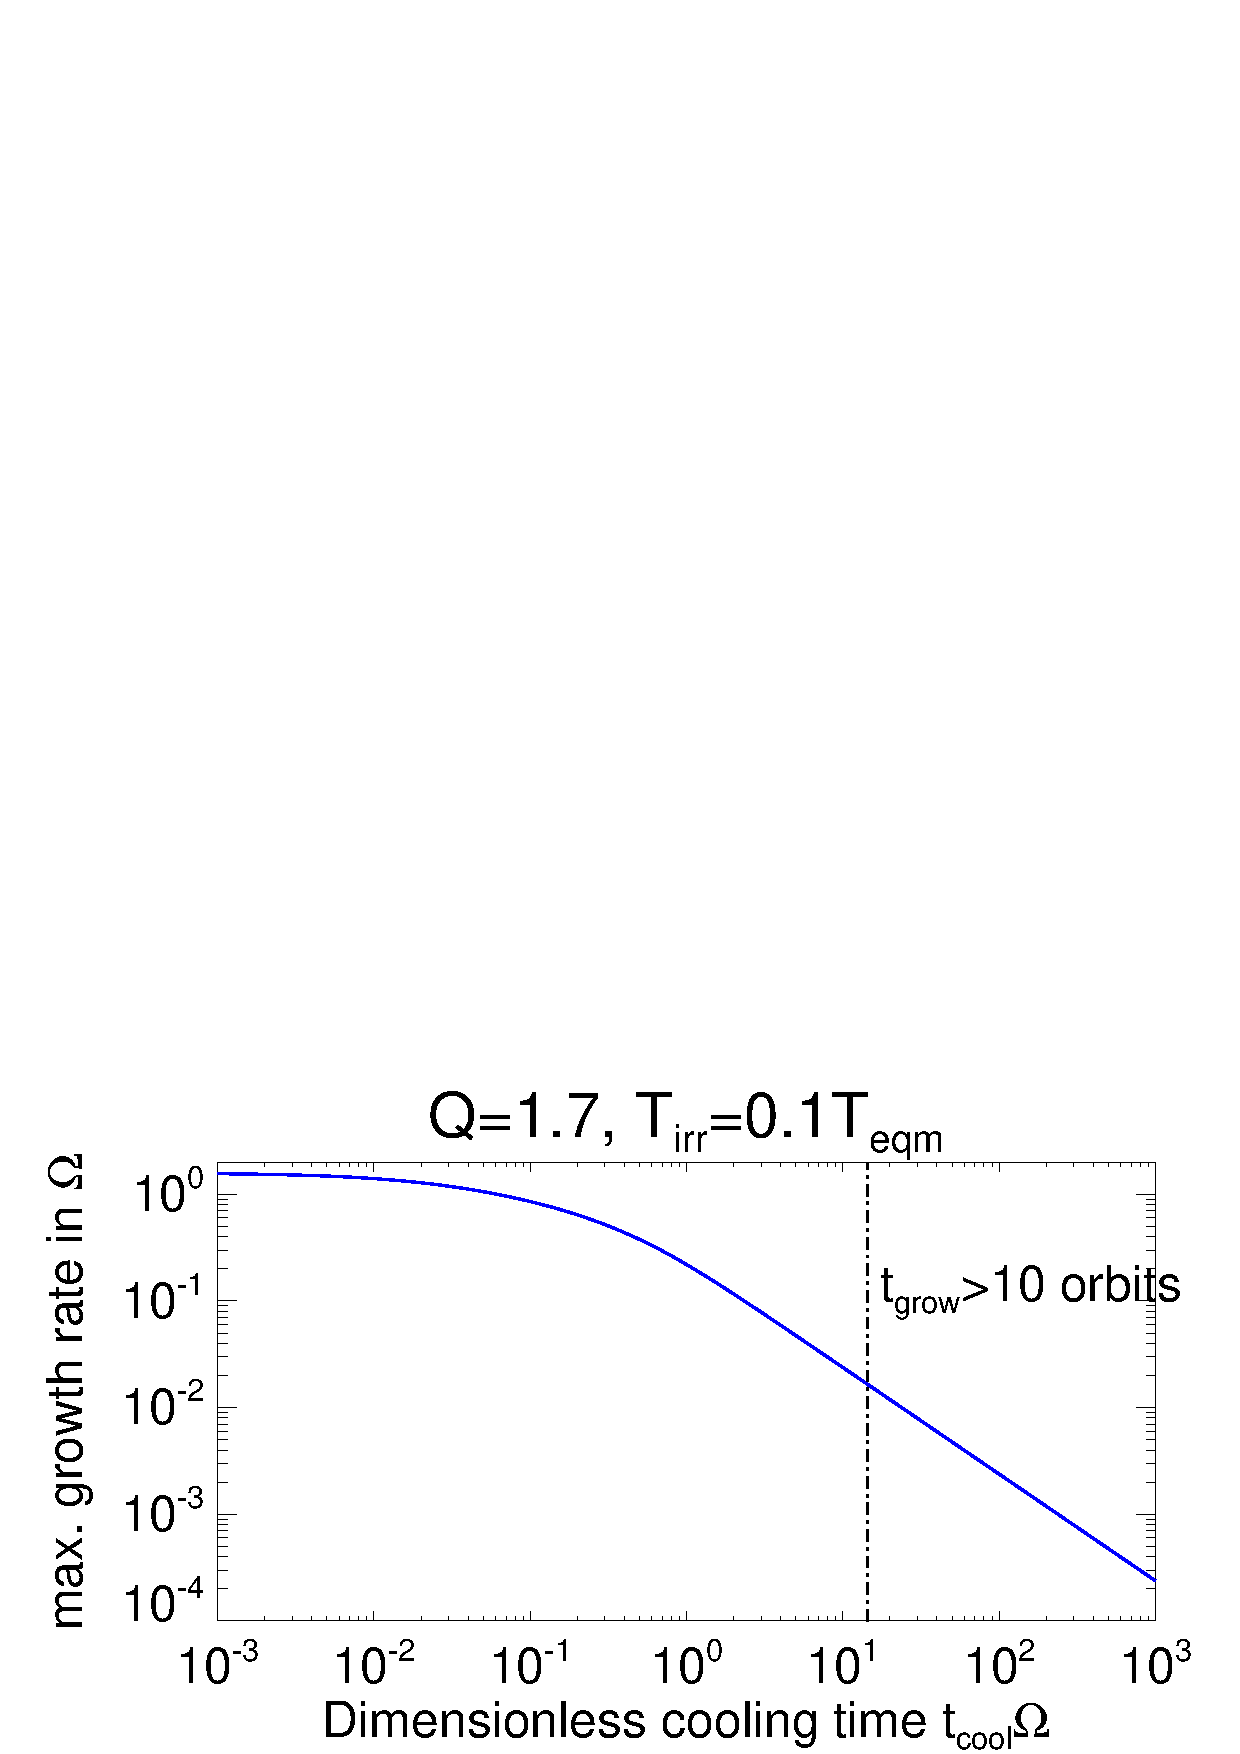
\includegraphics[width=\linewidth,clip=true,trim=0cm 0cm 0cm 0cm]{figures/2dinvisc_theta}
                \end{figure}
              \end{block}
              
            \begin{block}{{\Large Understanding (some) simulations}}
              \justifying
              \begin{figure}
                  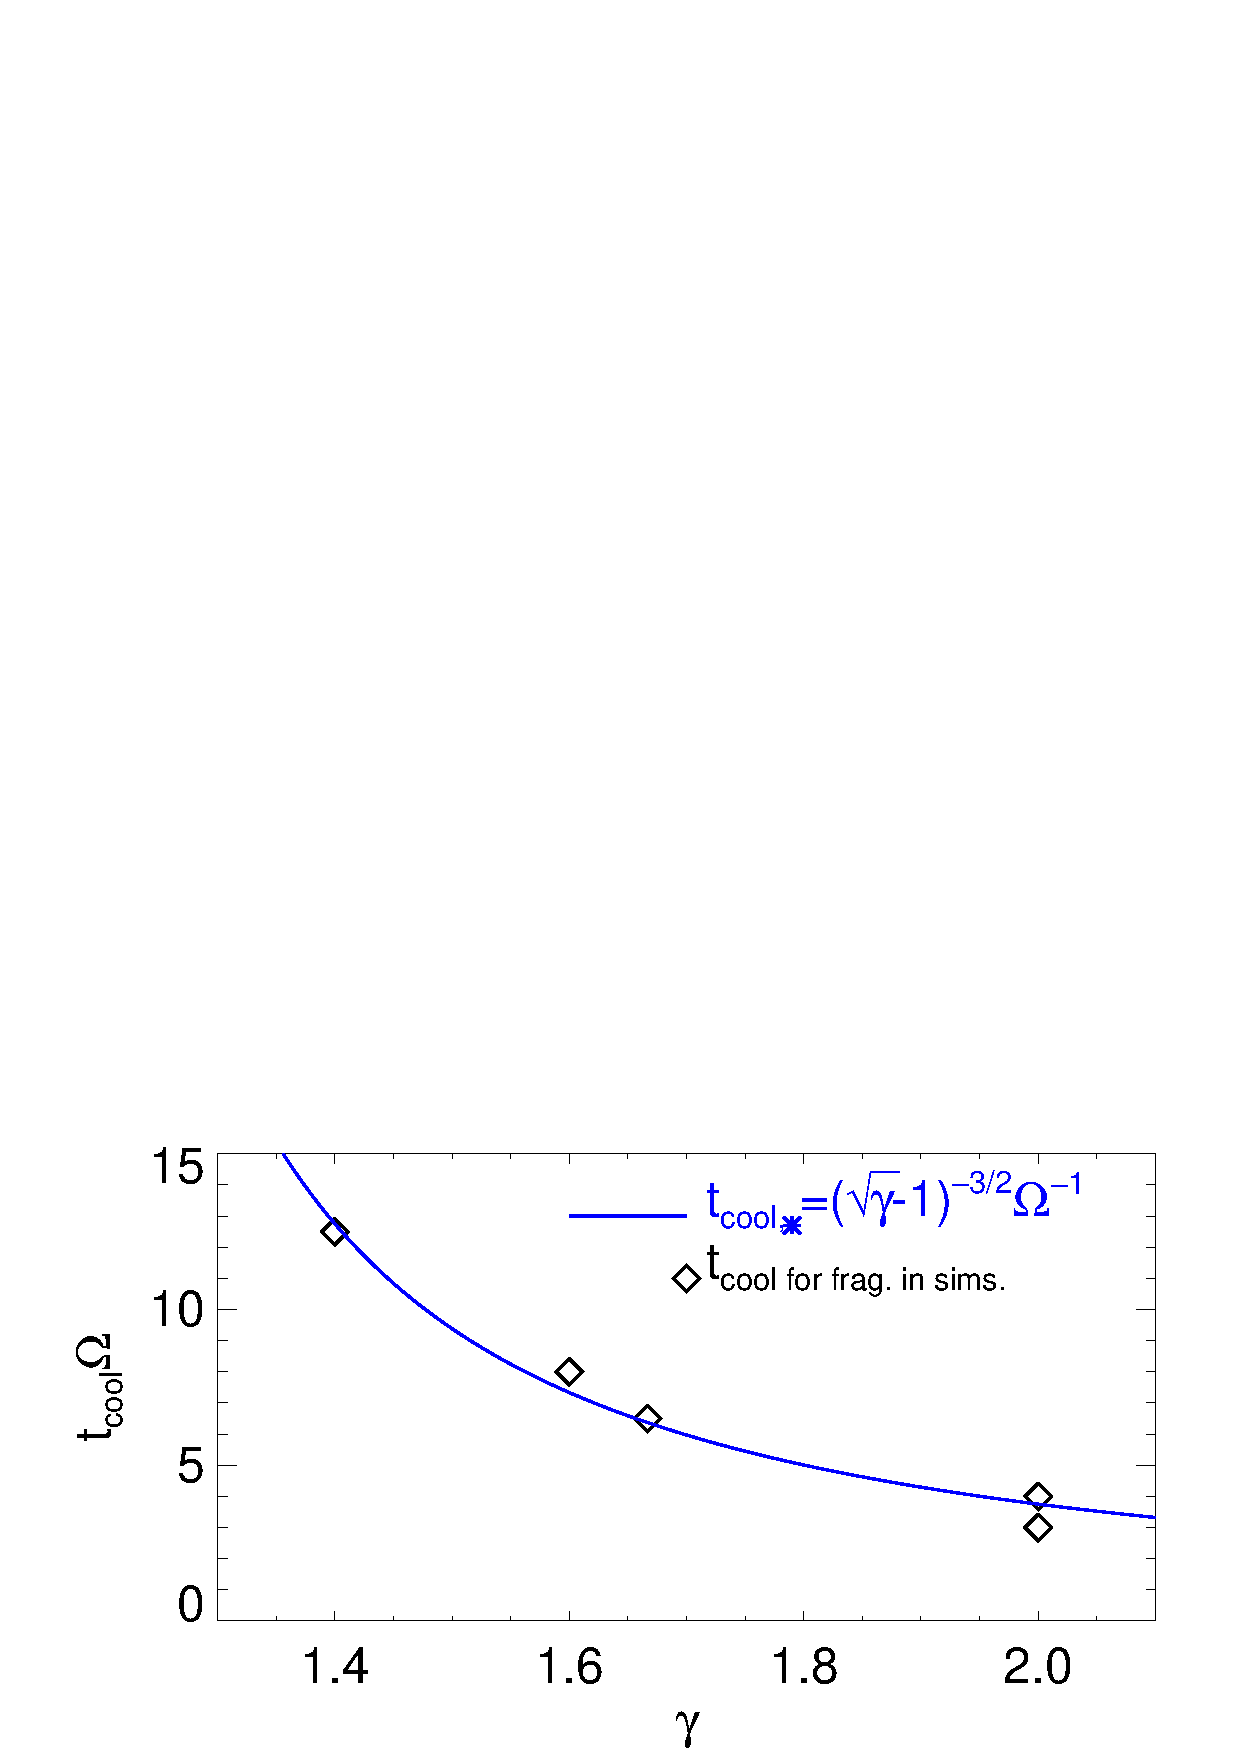
\includegraphics[width=\linewidth,clip=true,trim=0cm 0cm 0cm 1cm]{figures/tcool}
                \end{figure}
            \end{block}
            
            \begin{block}{{\Large Viscosity-driven GI}}
              \justifying
              \begin{figure}
                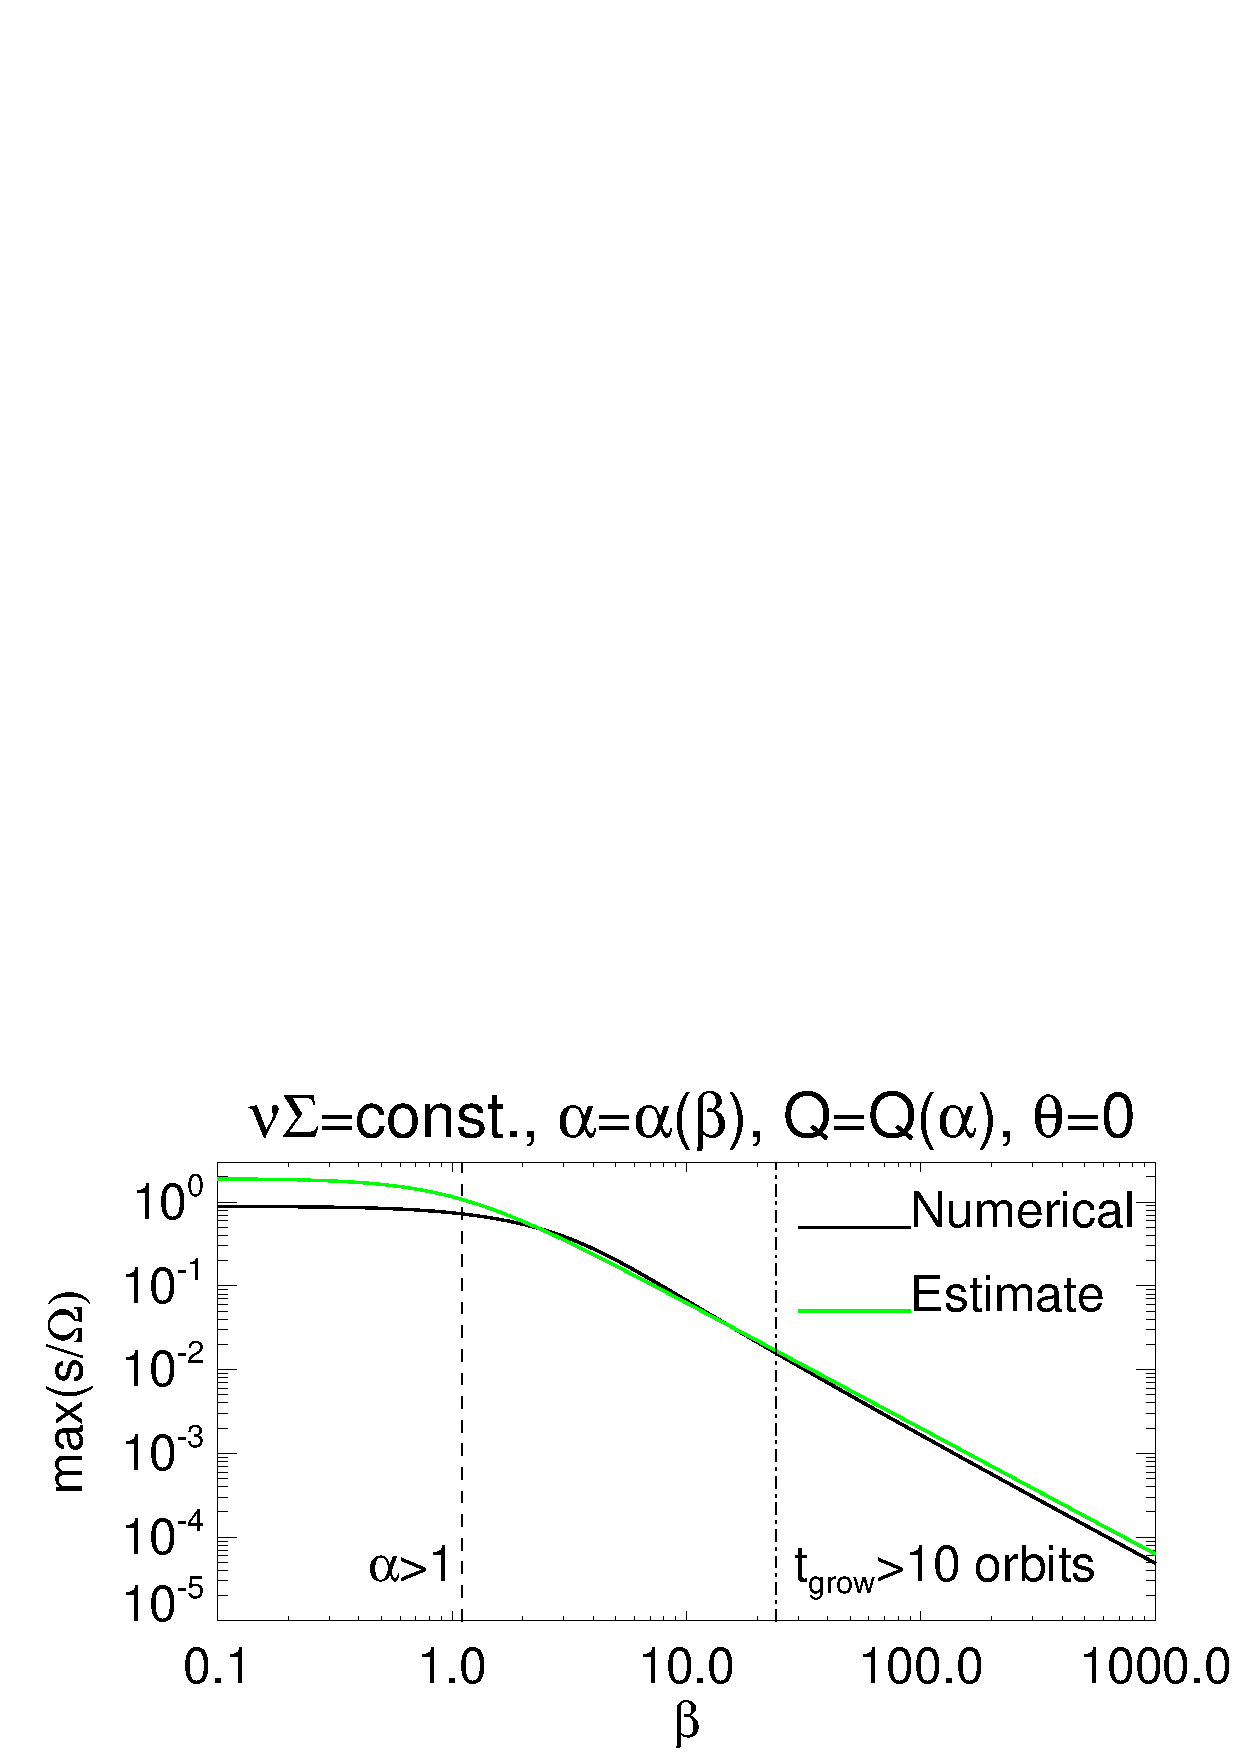
\includegraphics[width=\linewidth,clip=true,trim=0cm 0cm 0cm 0cm]{figures/result2d_gvisc}
              \end{figure}
            \end{block}
              
            \begin{block}{{\Large Application to protoplanetary disks}}
              \justifying
               \begin{figure}
                 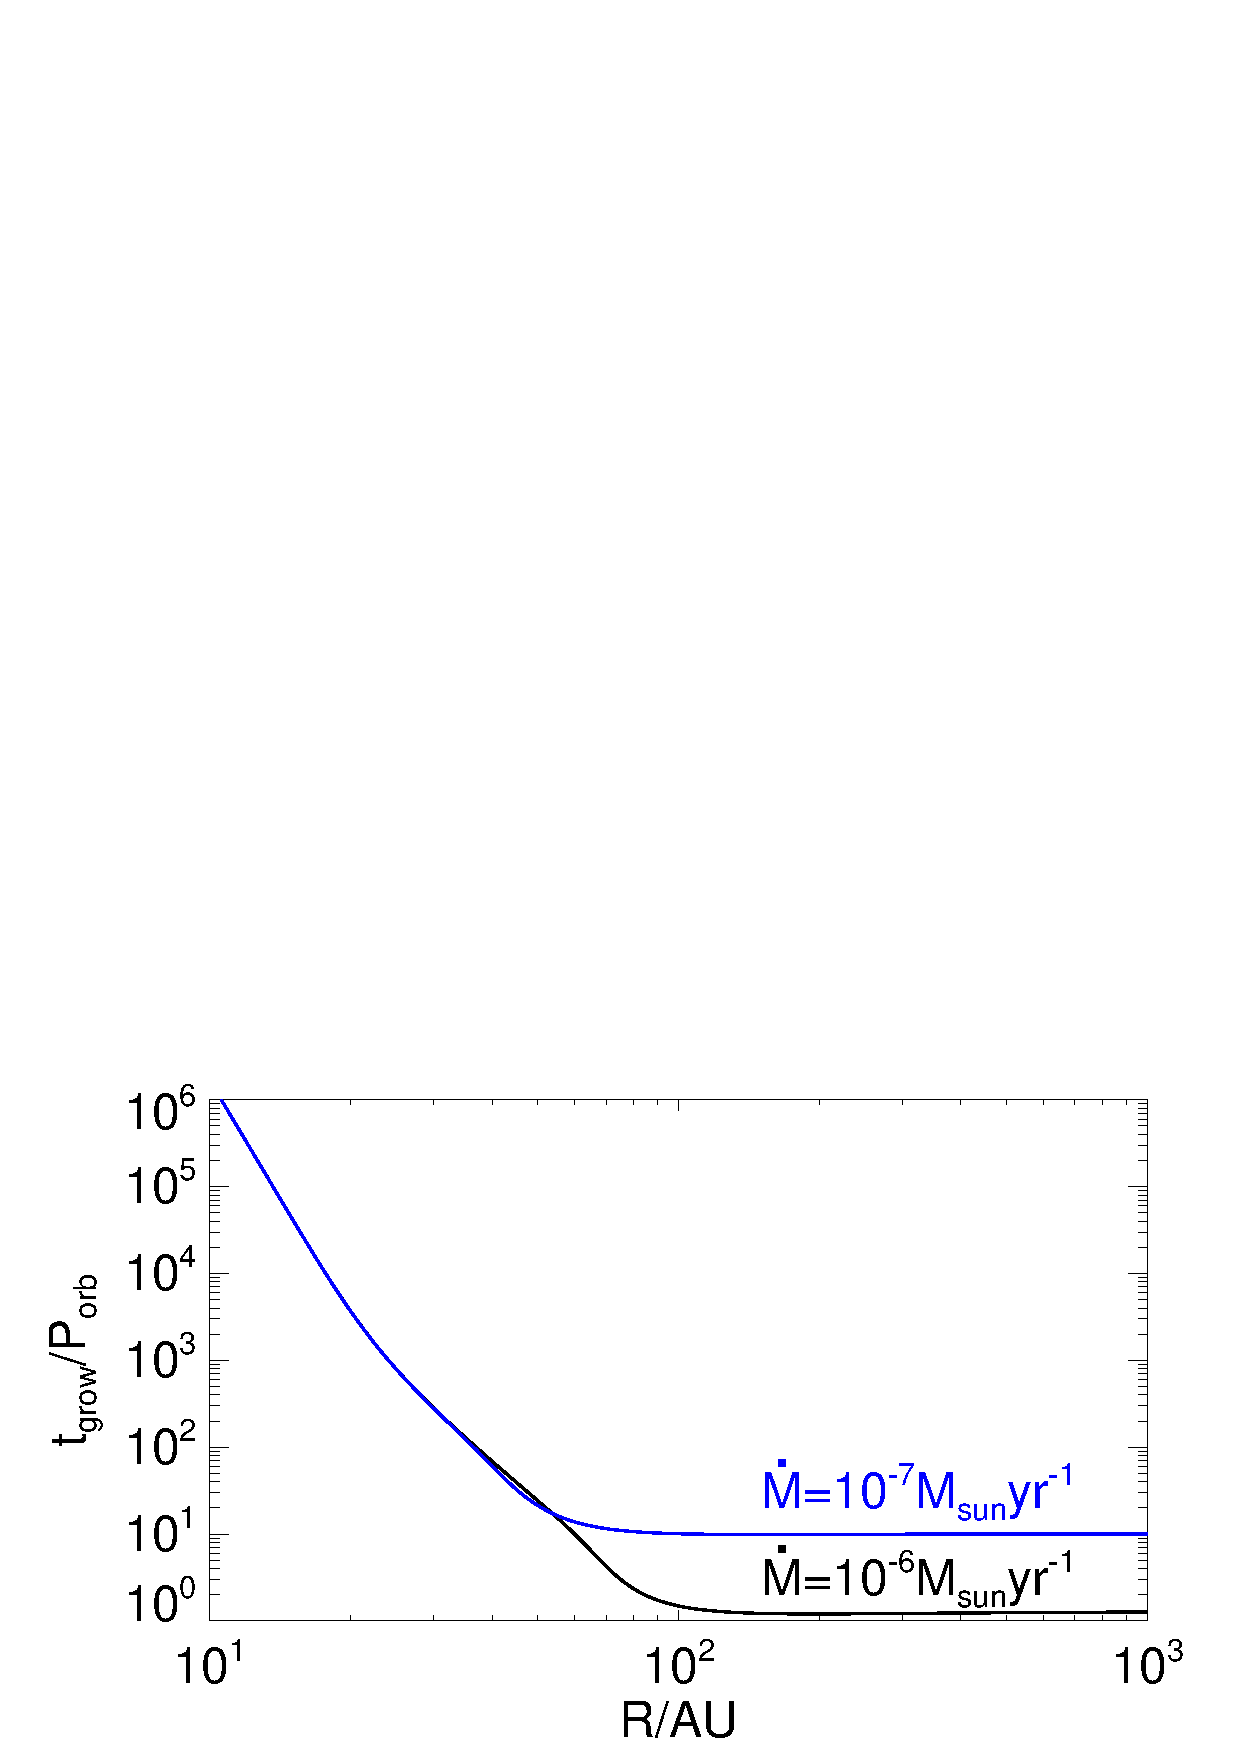
\includegraphics[width=\linewidth,clip=true,trim=0cm 0cm 0cm 0cm]{figures/compare_result_growth}
              \end{figure}
            \end{block}
            

              
            
              \vfill
              }
            \end{minipage}
          \end{beamercolorbox}
        \end{column}
        % ---------------------------------------------------------%
      % end the column
    \end{columns}
     % \begin{block}{\Large{Summary and discussion}}
     %           \justifying
     %            Large-scale spiral structures have been observed in
     %              the outer parts of transition disks. These could be
     %              due to unseen planets, but theoretical alternatives
     %              should be explored. We describe a 
     %              new but simple mechanism that can lead to the growth
     %              of one-armed spirals, or eccentric modes, in irradiated 
     %              astrophysical disks, which may be applicable to the outer
     %              parts of protoplanetary disks. We explain this new
     %              instability with linear density wave 
     %              theory, and confirm it through 2D and 3D
     %              hydrodynamic simulations. We find this mechanism can
     %              produce long-lived spiral structures. 
     %        \end{block}
    \vskip1ex
\end{frame}
\end{document}


%%%%%%%%%%%%%%%%%%%%%%%%%%%%%%%%%%%%%%%%%%%%%%%%%%%%%%%%%%%%%%%%%%%%%%%%%%%%%%%%%%%%%%%%%%%%%%%%%%%%
%%% Local Variables: 
%%% mode: latex
%%% TeX-PDF-mode: t
%%% End:
